\documentclass[conference]{IEEEtran}

\usepackage[utf8]{inputenc}
\usepackage[T1]{fontenc}
\usepackage{lmodern}
\usepackage{amsmath,amssymb}
\usepackage{booktabs}
\usepackage{array}
\usepackage{url}
\usepackage{cite}
\usepackage{graphicx}
\usepackage{listings}
\usepackage{xcolor}
\usepackage{hyperref}

\hypersetup{colorlinks=true,linkcolor=black,citecolor=black,urlcolor=black}

% Rapor hem teslim/rapor/ hem reports/ieee_keep_cull_rl_report/ altından derlenebilsin.
\graphicspath{{../sunum/grafikler/}{../../teslim/sunum/grafikler/}{teslim/sunum/grafikler/}}

\lstset{basicstyle=\ttfamily\footnotesize,breaklines=true,columns=fullflexible,
  keepspaces=true,frame=single,framesep=3pt,xleftmargin=2pt}

\renewcommand\IEEEkeywordsname{Anahtar Kelimeler}

\title{Süt Sığırcılığında İnek Bazında Elde~Tutma/Sürüden~Çıkarma Kararı için \\ Model-Free Pekiştirmeli Öğrenme: Empirik Stokastik Bir MDP Üzerinde \\ Q-Learning ve DQN'in Karşılaştırmalı Değerlendirmesi}

\author{
\IEEEauthorblockN{Artun Kara (255172008)}
\IEEEauthorblockA{Bilişim Sistemleri Mühendisliği\\ Kocaeli, Türkiye\\ artunankara@gmail.com}
}

\begin{document}
\maketitle

\begin{abstract}
Süt sığırcılığında her inek için aylık olarak verilen \emph{elde tutma (keep)} veya
\emph{sürüden çıkarma (cull)} kararı; ardışık, ödülü gecikmeli ve dinamiği belirsiz
bir sıralı karar problemidir. Bu çalışmada, gerçek hayvan kayıtlarından kestirilen
\emph{empirik ve stokastik} bir Markov Karar Süreci (MDP) ortamı kurulmuş ve karar
politikası, modeli bilmeyen (\emph{model-free}) iki pekiştirmeli öğrenme (RL) ajanıyla
öğrenilmiştir: tablo tabanlı Q-Learning ve derin Q-ağı (Stable-Baselines3 DQN). Ödül,
ABD~2025 ekonomik parametrelerinden türetilen ve kodla birebir eşleşen bir aylık kar
fonksiyonudur. Ajanlar; rastgele, keep-all, cull-all ve risk-eşiği temel
politikalarıyla (baseline) ve modeli bilen değer iterasyonu (value iteration, VI)
optimumuyla, beş tohum (seed) üzerinde ortalama$\pm$standart sapma bandıyla
karşılaştırılmıştır. Tam ölçekli koşuda Q-Learning $-204$, DQN $-270$ USD ortalama
episode getirisi elde ederek tüm baseline'ları belirgin biçimde geçmiş; Q-Learning,
model tabanlı VI optimumuyla ($-225$) istatistiksel olarak eşitlenmiştir (fark anlamlı değildir).
Tüm sonuçlar $\geq5$ tohum üzerinde tekrarlanabilir, ham loglardan doğrulanabilir ve
tek komutla yeniden üretilebilir.
\end{abstract}

\begin{IEEEkeywords}
pekiştirmeli öğrenme, Markov karar süreci, Q-learning, DQN, model-free,
sürü yönetimi, keep/cull, stokastik ortam
\end{IEEEkeywords}

\section{Giriş}
Süt sığırcılığı işletmelerinde sürü kompozisyonu, işletme kârlılığının en güçlü
belirleyicilerinden biridir. Bir ineğin sürüde tutulması; gelecekteki süt geliriyle,
artan hastalık ve üreme riskinin getirdiği maliyetler arasında bir denge gerektirir.
Bir ineğin sürüden çıkarılması ise anlık bir karkas/satış geliri sağlar, ancak yerine
yüksek maliyetli bir düve (replacement) konmasını zorunlu kılar. Bu karar tek seferlik
değildir: her ay, her hayvan için yeniden verilir ve bugünkü karar, hayvanın gelecekteki
durumunu ve dolayısıyla gelecekteki getiriyi doğrudan etkiler.

Bu rapor, problemi sıralı bir karar süreci olarak ele alır ve şu katkıları sunar:
(i) gerçek hayvan kayıtlarından kestirilen, geçişleri stokastik bir keep/cull MDP
ortamı; (ii) ekonomik parametrelerden türetilen ve kaynak kodla \emph{birebir} eşleşen
bir ödül mekanizması; (iii) iki model-free RL ajanının (tablo Q-Learning ve derin DQN)
çok-tohumlu, baseline ve model-tabanlı optimumla karşılaştırmalı değerlendirmesi;
(iv) tamamen tekrarlanabilir, ham loglardan doğrulanabilir bir deney hattı. Çalışmanın
hedefi, okuyucunun problemin neden RL gerektirdiğini, ortamın nasıl kurulduğunu, ödülün
neyi optimize ettiğini ve hangi yöntemin neden seçildiğini eksiksiz anlamasıdır.

\subsection{İlgili Çalışmalar}
İnek değiştirme (cow replacement) problemi, harekât araştırmasında onlarca yıldır dinamik
programlama (DP) ve Markov karar süreçleriyle incelenmiştir; Kristensen'in hiyerarşik
Markov süreçleri \cite{kristensen} ve Cabrera'nın ekonomik replacement modelleri
\cite{cabrera} bu geleneğin temsilcileridir. Bu klasik çalışmalar geçiş ve verim
dağılımlarını çoğunlukla \emph{varsayımsal parametrik} biçimde alıp modeli bilen DP ile
çözer. Bu çalışmanın ayırt edici yanı; geçişleri \emph{gerçek aylık kayıtlardan empirik}
kestirmesi, kararı \emph{model-free} RL (Q-Learning, DQN) ile öğrenmesi, denetimli bir
culling-risk skorunu duruma katması ve sonuçları $\geq5$ tohumla tekrarlanabilir biçimde
raporlamasıdır. Genel iş akışı Şekil~\ref{fig:pipeline}'de özetlenmiştir.

\begin{figure*}[t]
\centering
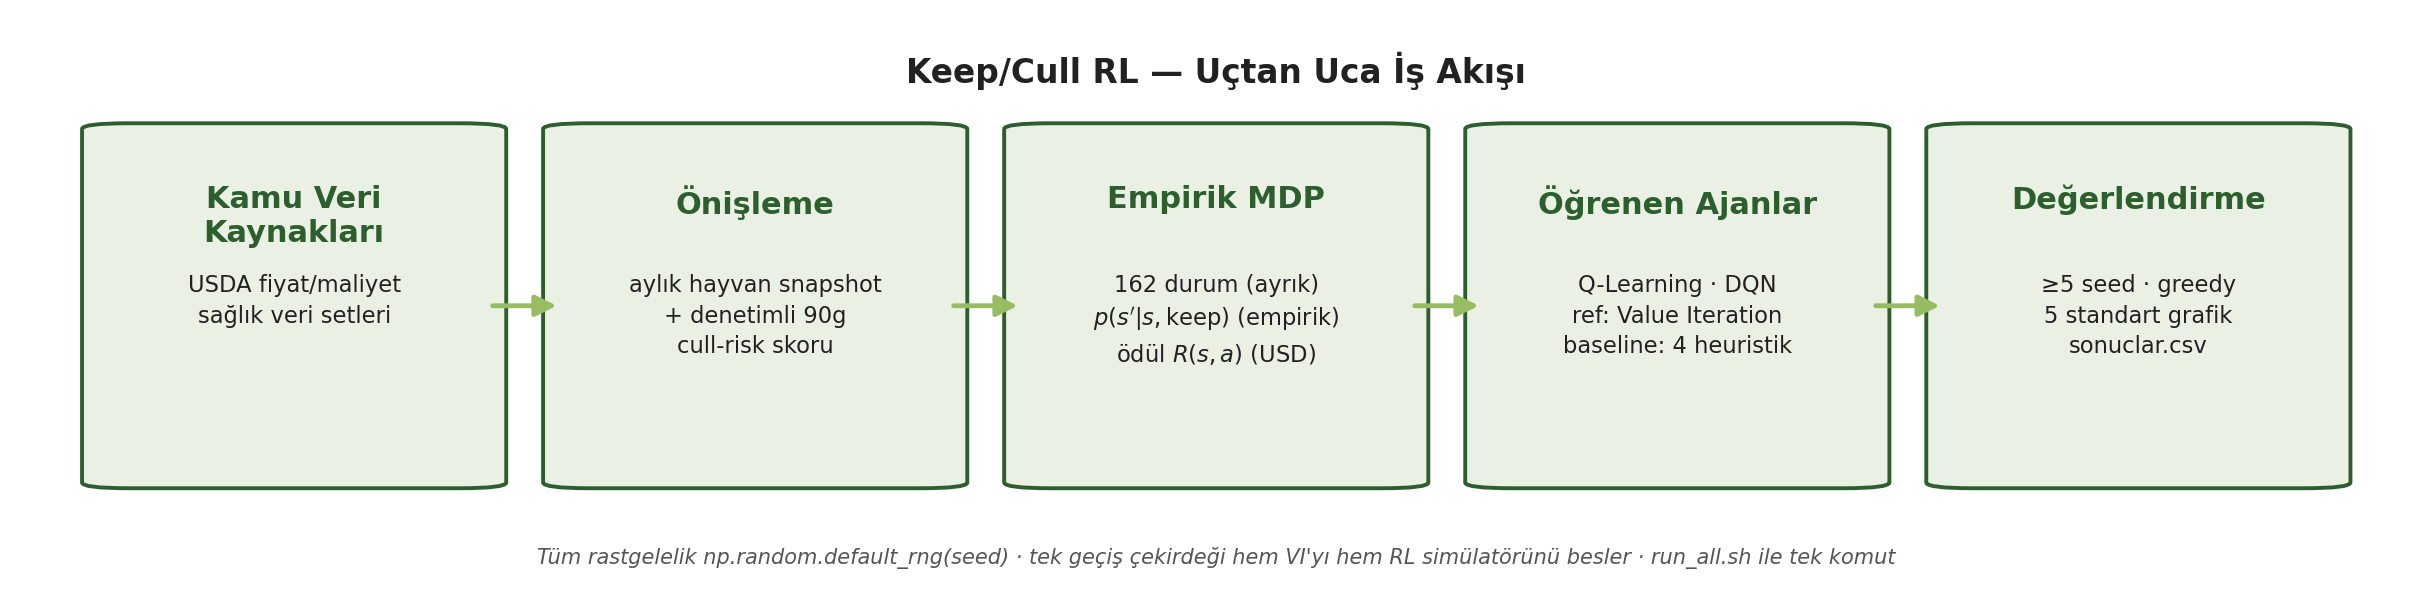
\includegraphics[width=0.96\textwidth]{00_pipeline.png}
\caption{Uçtan uca iş akışı: kamu verisi $\rightarrow$ aylık snapshot ve denetimli risk
skoru $\rightarrow$ empirik stokastik MDP (durum/geçiş/ödül) $\rightarrow$ model-free
ajanlar (VI referans, heuristik baseline) $\rightarrow$ çok-tohumlu değerlendirme.}
\label{fig:pipeline}
\end{figure*}

\section{Arka Plan ve Neden Pekiştirmeli Öğrenme?}
\subsection{Markov Karar Süreci}
Problem $\langle \mathcal{S}, \mathcal{A}, P, R, \gamma\rangle$ beşlisiyle modellenir:
$\mathcal{S}$ durum kümesi, $\mathcal{A}=\{\text{keep},\text{cull}\}$ aksiyon kümesi,
$P(s'\mid s,a)$ geçiş olasılığı, $R(s,a)$ ödül ve $\gamma=0.97$ iskonto faktörüdür.
Amaç, beklenen iskontolu getiriyi $\mathbb{E}\big[\sum_t \gamma^t R(s_t,a_t)\big]$
enbüyükleyen bir $\pi(a\mid s)$ politikasıdır.

\subsection{Neden RL? (zorunlu gerekçe)}
Problemin RL gerektirdiği dört ölçütle gösterilir:
\begin{itemize}
\item \textbf{Ardışıklık:} \texttt{keep} aksiyonu hayvanı bir sonraki aylık duruma
taşır (laktasyon ilerler, verim ve risk değişir); karar geleceği etkiler.
\item \textbf{Gecikmeli ödül:} Tutmanın değeri, gelecekteki süt gelirinden birikmiş
sağlık/üreme riskinin çıkarılmasıdır; bu ancak ileride gerçekleşir.
\item \textbf{Belirsiz dinamik ve büyük uzay:} Geçiş kuralı analitik değil, gerçek
kayıtlardan empirik olarak kestirilmiştir; 162 ayrık durum ve stokastik geçişler içerir.
\item \textbf{Daha ucuz alternatif yok:} Ortam stokastik olduğundan (Bölüm
\ref{sec:transition}) A$^\ast$/BFS gibi tek-hedefli en kısa yol yöntemleri uygulanamaz;
basit risk-eşiği kuralı denenmiş ve RL ajanlarının gerisinde kalmıştır.
\end{itemize}
Ortam statik/deterministik küçük bir ızgara değildir; bu nedenle baseline karşılaştırması
zorunlu olmamakla birlikte RL kazancını ölçmek için dahil edilmiştir.

\subsection{Neden Model-Free?}
Çalışmada modeli bilen bir referans (value iteration) bilinçli olarak tutulmuştur;
ancak teslim edilen \emph{öğrenen} ajanlar model-free'dir. Üç gerekçe öne çıkar.
Birincisi, dersin amacı öğrenmeyi (öğrenme/eval eğrileri, keşif--sömürü dengesi)
göstermektir; model-free ajanlar bu dinamiği doğrudan üretir. İkincisi, model-free
yöntemler karar anında tam geçiş modeline ihtiyaç duymadan örneklenmiş etkileşimden
öğrenir; bu, modelin bilinmediği veya çok büyük olduğu gerçek dünya koşullarına
genelleşir. Üçüncüsü, model-free Q-Learning bu ortamda model-tabanlı VI optimumuna
istatistiksel olarak eşitlenmiştir (Bölüm \ref{sec:results}); aradaki fark, sonlu-örneklem
Monte-Carlo değerlendirme gürültüsü içindedir (eşli $t$-testi $p\approx0.37$; bir tohumda VI
öndedir). VI, simülatörle aynı geçiş çekirdeğinin optimumu olduğundan gerçek tavandır; bu
sonuç, modeli hiç kullanmayan bir ajanın geçiş modelini bilmeden model-tabanlı optimuma
ulaşabildiğini gösterir.

\section{Ortam ve MDP Formülasyonu}
\subsection{Durum (State)}
Her hayvan-ay snapshot'ı, aşağıdaki bileşenlerin ayrıklaştırılmasıyla bir \emph{durum
kovasına} (\texttt{state\_bucket\_exact}) eşlenir:
laktasyon evresi, parite grubu, DIM (laktasyon günü) bandı, süt seviyesi bandı, süt
trendi bandı, sağlık risk bandı ve denetimli modelden gelen 90 günlük culling-risk bandı.
Bu ayrıklaştırma 162 ulaşılabilir durum üretir. Süt trendi ve risk bandı gibi bileşenler,
geçmiş bilgisinin bir özetini duruma taşıyarak Markov varsayımını güçlendirir.

\subsection{Aksiyon (Action)}
Aksiyon uzayı iki ayrık seçenekten oluşur: \texttt{keep} (0, terminal değil) ve
\texttt{cull} (1, terminal). Gymnasium ortamında bu
\texttt{spaces.Discrete(2)} ile tanımlıdır.

\subsection{Ödül Mekanizması (kod ile birebir)}
\label{sec:reward}
Ödül, bir aylık net ekonomik kârı temsil eder. Parametreler
\texttt{reward\_baseline\_us\_2025.csv} dosyasından gelir; süt fiyatı ve bakım maliyeti
USDA~2025 kaynaklıdır, kalan dört parametre prototip varsayımıdır (Bölüm
\ref{sec:limitations}). \textbf{Keep} ödülü, ineği bir ay daha tutmanın net getirisini
modeller: süt geliri eksi bakım, sağlık riski, üreme riski ve beklenen culling riski
maliyetleri (kaynak: \texttt{kod/env/rl\_mdp\_utils.py:120}):
\begin{equation}
R_{\text{keep}}(s) = \underbrace{m\,d\,p}_{\text{süt geliri}}
- \underbrace{c_b\,d}_{\text{bakım}}
- C_{\text{sağlık}} - C_{\text{üreme}} - C_{\text{bek-cull}}
\end{equation}
\begin{align}
C_{\text{sağlık}} &= c_t\!\left(\tfrac{1}{3}n_{h} + 0.25\,\mathbf{1}_{\text{mast}} + 0.25\,\mathbf{1}_{\text{top}} + 0.15\,\mathbf{1}_{\text{hücre}}\right)\\
C_{\text{üreme}} &= c_i\max(n_{s}-2,0) + c_i\,\mathbf{1}_{[\text{gebe}<0.5\,\wedge\,\text{DIM}>150]}\\
C_{\text{bek-cull}} &= 0.25\;p^{30}_{\text{cull}}\;c_r
\end{align}
\textbf{Cull} ödülü, hayvanı bugün çıkarmanın net getirisidir: karkas/satış değeri eksi
düve maliyeti (kaynak: \texttt{kod/env/rl\_mdp\_utils.py:76}):
\begin{equation}
R_{\text{cull}}(s) = v_c - c_r - c_{\text{disp}},\qquad c_{\text{disp}}=0
\end{equation}
Sezgisel olarak: $R_{\text{keep}}$ yüksek sütlü, sağlıklı, düşük riskli ineklerde
pozitife yaklaşır; risk ve maliyet biriktikçe küçülür. $R_{\text{cull}}$ ise sabit bir
taban getiridir ($v_c-c_r$). Ajan, bu iki getirinin \emph{gelecekteki} sonuçlarını
iskontolayarak karşılaştırmayı öğrenir. Sembollerin değer ve kod karşılıkları Tablo
\ref{tab:reward}'de verilmiştir; rapordaki LaTeX ile kod birebir aynıdır.

\begin{table}[t]
\caption{Ödül sembolleri, değerleri ve kaynak kod satırları.}
\label{tab:reward}
\centering\footnotesize
\begin{tabular}{@{}clr l@{}}
\toprule
Sembol & Anlam & Değer & Kod (\texttt{rl\_mdp\_utils.py}) \\
\midrule
$m$ & günlük süt (kg) & durum & \texttt{:89--90} \\
$d$ & ay/gün & 30.4375 & \texttt{config: days\_in\_month} \\
$p$ & süt fiyatı & 0.4668 & \texttt{:90} \\
$c_b$ & günlük bakım & 8.5337 & \texttt{:91} \\
$c_t$ & tedavi & 150 & \texttt{:96--105} \\
$c_i$ & tohumlama & 35 & \texttt{:109--113} \\
$c_r$ & replacement & 2500 & \texttt{:115--119, 76} \\
$v_c$ & cull satışı & 1200 & \texttt{:76} \\
$p^{30}_{\text{cull}}$ & 30g risk (denetimli) & --- & \texttt{:115--119} \\
\bottomrule
\end{tabular}
\end{table}

\textbf{Sayısal örnek.} Sağlıklı, yüksek verimli bir inek ($m\!=\!35$~kg, sağlık olayı yok,
gebe, DIM$=\!80$, $p^{30}_{\text{cull}}\!=\!0.05$) için
$R_{\text{keep}}=497.3-259.7-31.3=+206.3$ USD iken aynı ay
$R_{\text{cull}}=1200-2500=-1300$ USD'dir: tutmak açıkça baskındır. Buna karşın düşük
verimli, hasta bir inek ($m\!=\!12$, mastitis ve topallık, $n_h\!=\!3$, açık, DIM$=\!200$,
servis$=\!4$, $p^{30}_{\text{cull}}\!=\!0.40$) için
$R_{\text{keep}}=170.5-259.7-225-105-250=-669.2$ USD olur; bu anlık değer hâlâ cull
tabanından ($-1300$) iyidir. Ancak böyle bir hayvanı tutmak ardışık olarak daha kötü
durumlara yol açar ve bu kötü ayların \emph{iskontolu toplamı} tek seferlik $-1300$'ün
altına inebilir; ajan, tam da bu \emph{gelecek} hesabı yüzünden bazı durumlarda cull'u
seçer. Bu, cull'un nadiren anlık olarak yeterli olduğunu fakat değerinin gelecekteki
trajektoriden geldiğini gösterir.

\subsection{Geçiş: Stokastik ve Empirik}
\label{sec:transition}
\texttt{keep} aksiyonundan sonraki durum, gerçek kayıt frekanslarından kurulan empirik
bir dağılımdan örneklenir (kaynak: \texttt{kod/env/rl\_experiment\_utils.py:161}):
\begin{lstlisting}
selected = outcomes[int(
    rng.choice(len(outcomes), p=probabilities))]
\end{lstlisting}
162 durumun 120'sinde ($\%74$) \texttt{keep} altında birden çok olası $s'$ vardır; örneğin
bir başlangıç durumu üç farklı sonraki duruma her biri $p\!=\!0.333$ olasılıkla geçer.
Bu, ortamın \emph{tanım gereği stokastik} olduğunu kanıtlar. \texttt{cull} ise
deterministik terminaldir. Tüm rastgelelik \texttt{np.random.default\_rng(seed)} ile
yönetilir; eski Gym API'si ve \texttt{np.random.seed/choice} kullanılmaz.

\textbf{Modelin kuruluşu.} Empirik geçiş modeli, aynı hayvanın ardışık aylık
snapshot'ları arasındaki gözlenen $(s,\text{keep},s')$ geçişleri sayılarak kurulur;
olasılık basit göreli frekanstır (\texttt{count/total\_count}, düzleştirme yok). Bir
durumun tam-kova desteği eşiğin altındaysa ($<\!5$), tahmin seyreklikten gürültülenmesin
diye model daha kaba kovalara \emph{geri-düşer}
(exact $\rightarrow$ risk'siz $\rightarrow$ evre+parite $\rightarrow$ global). Kritik
olarak bu \emph{tek} geçiş çekirdeği hem değer iterasyonunu hem de RL simülatörünü besler;
dolayısıyla VI ile ajanlar arasında bir model uyuşmazlığı yoktur ve Bölüm
\ref{sec:results}'teki karşılaştırma aynı dinamik üzerinde adildir.

\section{Yöntemler}
Tablo \ref{tab:methods} dört yaklaşımı özetler. \emph{Öğrenen} ajanlar model-free'dir;
VI optimum referans (tavan), heuristikler ise baseline'dır.

\begin{table}[t]
\caption{Yöntemler ve rolleri.}
\label{tab:methods}
\centering\footnotesize
\begin{tabular}{@{}p{2.5cm} p{2.6cm} p{2.4cm}@{}}
\toprule
Yöntem & Tür & Rol \\
\midrule
Tablo Q-Learning & model-free, off-policy & Ana ajan \\
SB3 DQN & model-free, off-policy, replay & Ana ajan (derin) \\
Value Iteration & model-based exact & Optimum referans \\
keep/cull/random/risk & heuristik & Baseline \\
\bottomrule
\end{tabular}
\end{table}

\textbf{Tablo Q-Learning} (off-policy). Davranış politikası $\varepsilon$-greedy'dir
(\texttt{kod/rl\_core.py:309}); güncelleme hedefi ise açgözlü
$r+\gamma\max_{a'}Q(s',a')$'dir (\texttt{:321}). Veriyi üreten politika ile
iyileştirilen politikanın farklı olması, yöntemi off-policy yapar. SARSA'dan tek satırlık
farkı, hedefte davranışın seçtiği $a'$ yerine $\max_{a'}$ kullanılmasıdır.

\textbf{SB3 DQN} (off-policy, derin). Gözlem, durum metadata'sından kurulan yoğun bir
sayısal vektördür (one-hot $+$ z-normalizasyon). DQN bir \emph{replay buffer}
(\texttt{kod/rl\_core.py:474}) ve hedef ağ kullanır; tekrar arabelleği, geçmiş
politikaların ürettiği geçişleri yeniden kullandığından yöntem tanımı gereği off-policy'dir.

\textbf{Value Iteration} empirik geçiş ve ödül tablolarından Bellman optimal denklemini
çözerek tavan referansı verir. \textbf{Baseline'lar} eğitimsizdir: \texttt{keep\_all},
\texttt{cull\_all}, \texttt{random} ($p_{\text{cull}}\!=\!0.05$) ve risk-eşiği
($p^{90}_{\text{cull}}\!\geq\!0.35$).

\section{Deneysel Kurulum}
Tüm eğitim ve değerlendirme beş tohum üzerinde tekrarlanır:
$\{42,123,2024,7,99\}$ ($\geq5$). \texttt{full} profilinde DQN 100k adım, Q-Learning 4000
episode boyunca eğitilir; iskonto $\gamma=0.97$, VI yakınsama toleransı $10^{-4}$.
Değerlendirme \emph{deterministik/açgözlü} politikayla, tohum başına 500 episode
koşularak yapılır; ortam stokastik olduğundan her değerlendirme bir dağılımdır.
Tekrarlanabilirlik için bağımlılıklar \texttt{==} ile sabitlenmiş, rastgelelik tohumlanmış
ve tüm hat tek komutla (\texttt{run\_all.sh}) üretilebilir kılınmıştır. Raporda anlatılan
her deneyin ham logu \texttt{sonuclar/loglar/} altında bulunur ve grafikler bu loglardan
doğrulanabilir. Eğitim hiperparametreleri Tablo~\ref{tab:hyper}'de toplanmıştır.

\begin{table}[t]
\caption{Eğitim hiperparametreleri (\texttt{full} profil).}
\label{tab:hyper}
\centering\footnotesize
\begin{tabular}{@{}l c c@{}}
\toprule
Parametre & Q-Learning & DQN \\
\midrule
İskonto $\gamma$ & 0.97 & 0.97 \\
Eğitim bütçesi & 4000 episode & 100k adım \\
Öğrenme oranı & $\alpha=0.18$ & $5\times10^{-4}$ \\
Keşif $\varepsilon$ & $0.35\!\to\!0.03$ (decay 0.999) & frac $0.35$, son $0.05$ \\
Replay buffer & --- & $10^5$ \\
\texttt{learning\_starts} & --- & 5000 \\
Batch boyutu & --- & 32 \\
\texttt{train\_freq} & --- & 4 adım \\
Hedef ağ güncel. & --- & 1000 adım \\
Mimari & tablo $|S|\!\times\!2$ & MLP [64,\,64] \\
\bottomrule
\end{tabular}
\end{table}

\section{Bulgular ve Tartışma}
\label{sec:results}
Tablo \ref{tab:results}, beş tohum üzerinde ortalama$\pm$standart sapma getirileri
özetler. Her iki ajan da tüm baseline'ları belirgin biçimde geçmiştir. DQN tohumlar
arasında oldukça kararlıdır (std~20). Q-Learning'in ortalama getirisi ($-204$), VI
optimumuyla ($-225$) istatistiksel olarak ayırt edilemezdir: aradaki fark, tohum/episode
değerlendirme gürültüsü içindedir (eşli $t$-testi $p\approx0.37$; bir tohumda VI öndedir).
Dolayısıyla VI gerçek tavandır ve Q-Learning onu geçmez, gürültü içinde ona ulaşır. Ayrıca
getiri dağılımı sağa çarpıktır (Q-Learning medyan $-556$, ortalama $-204$): ajan,
\texttt{keep\_all}'ın sol-kuyruk felaket episode'larını cull ederek beklenen getiriyi
(RL'in optimize ettiği ortalama) iyileştirir.

\begin{table}[t]
\caption{Sonuçlar (seed ort.$\pm$std, \texttt{full}; yüksek=iyi).}
\label{tab:results}
\centering\footnotesize
\begin{tabular}{@{}l l r r r@{}}
\toprule
Politika & Tür & Getiri & Std & Cull \\
\midrule
\textbf{qlearning} & ajan & $\mathbf{-204}$ & 30 & 0.72 \\
mdp\_value\_iteration & referans & $-225$ & 42 & 0.45 \\
\textbf{dqn} & ajan & $\mathbf{-270}$ & 20 & 0.82 \\
risk\_threshold & baseline & $-385$ & 53 & 0.85 \\
keep\_all & baseline & $-428$ & 34 & 0.00 \\
random\_policy & baseline & $-964$ & 56 & 0.75 \\
cull\_all & baseline & $-1300$ & 0 & 1.00 \\
\bottomrule
\end{tabular}
\end{table}

\subsection{Öğrenme Eğrisi (Şekil \ref{fig:learn})}
Her iki ajanın \emph{eğitim episode getirisi}, tohum ortalamasında istikrarlı biçimde
yükselir: Q-Learning $\approx\!-1000$'den $\approx\!-450$'ye, DQN $\approx\!-1200$'den
$\approx\!-400$'e ilerler. Tablo ajanı daha hızlı ve oturmuş bir eğri verirken, DQN ilk
binlerce adımda daha gürültülüdür; bunun nedeni fonksiyon yaklaşımı ve tekrar
arabelleğinin başlangıçta yarattığı değişkenliktir. Gölgeli std bandı, getirinin tek bir
şanslı koşunun değil, beş tohum üzerinde sistematik bir öğrenmenin ürünü olduğunu
gösterir. Pratik çıkarım, y-ekseninin anlık ödül değil episode getirisi olması sayesinde
öğrenmenin açıkça görünür olmasıdır.

\begin{figure*}[t]
\centering
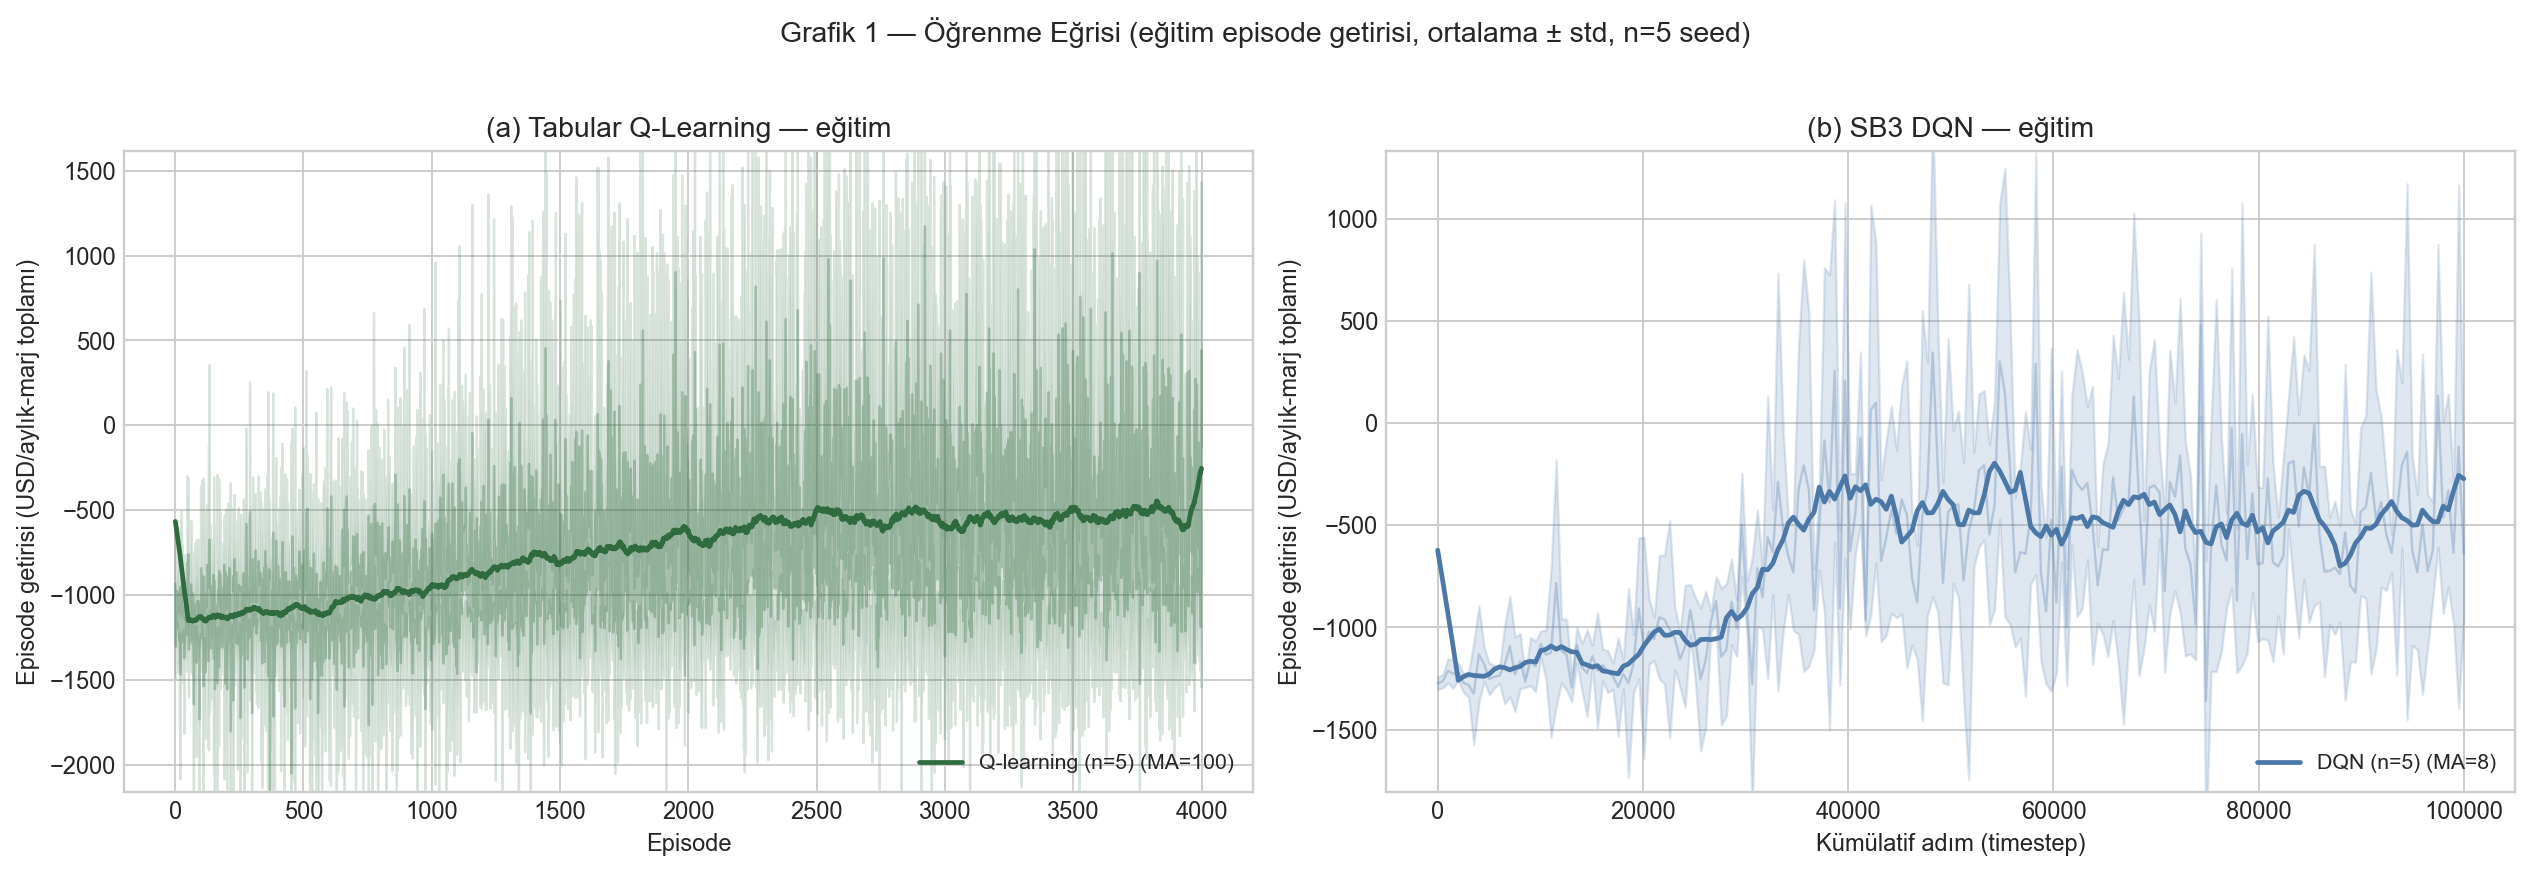
\includegraphics[width=0.92\textwidth]{01_ogrenme_egrisi.png}
\caption{Öğrenme eğrisi: eğitim episode getirisi (y) -- episode/timestep (x);
$n\!=\!5$ tohum, ortalama$\pm$std bandı ve hareketli ortalama.}
\label{fig:learn}
\end{figure*}

\subsection{Test/Değerlendirme Eğrisi (Şekil \ref{fig:eval})}
Deterministik/açgözlü değerlendirme getirisi eğitimle birlikte iyileşir ve yeşil kesik
çizgiyle gösterilen VI optimum referansına yaklaşır ve onunla örtüşür (istatistiksel olarak ayırt edilemez).
Değerlendirme eğrisi, keşif kapalı olduğu için eğitim eğrisinden daha az gürültülüdür;
bu, eğitim eğrisinin tek başına politika kalitesinin kanıtı sayılamayacağını gösterir.
Açgözlü koşu, öğrenilen değer fonksiyonunun fiilî politika kalitesini ölçer; ortam
stokastik olduğundan değerlendirme de bir dağılımdır. Sonuç olarak öğrenilen politikalar,
görülmemiş episode başlangıçlarında da tutarlı getiri üretmektedir.

\begin{figure*}[t]
\centering
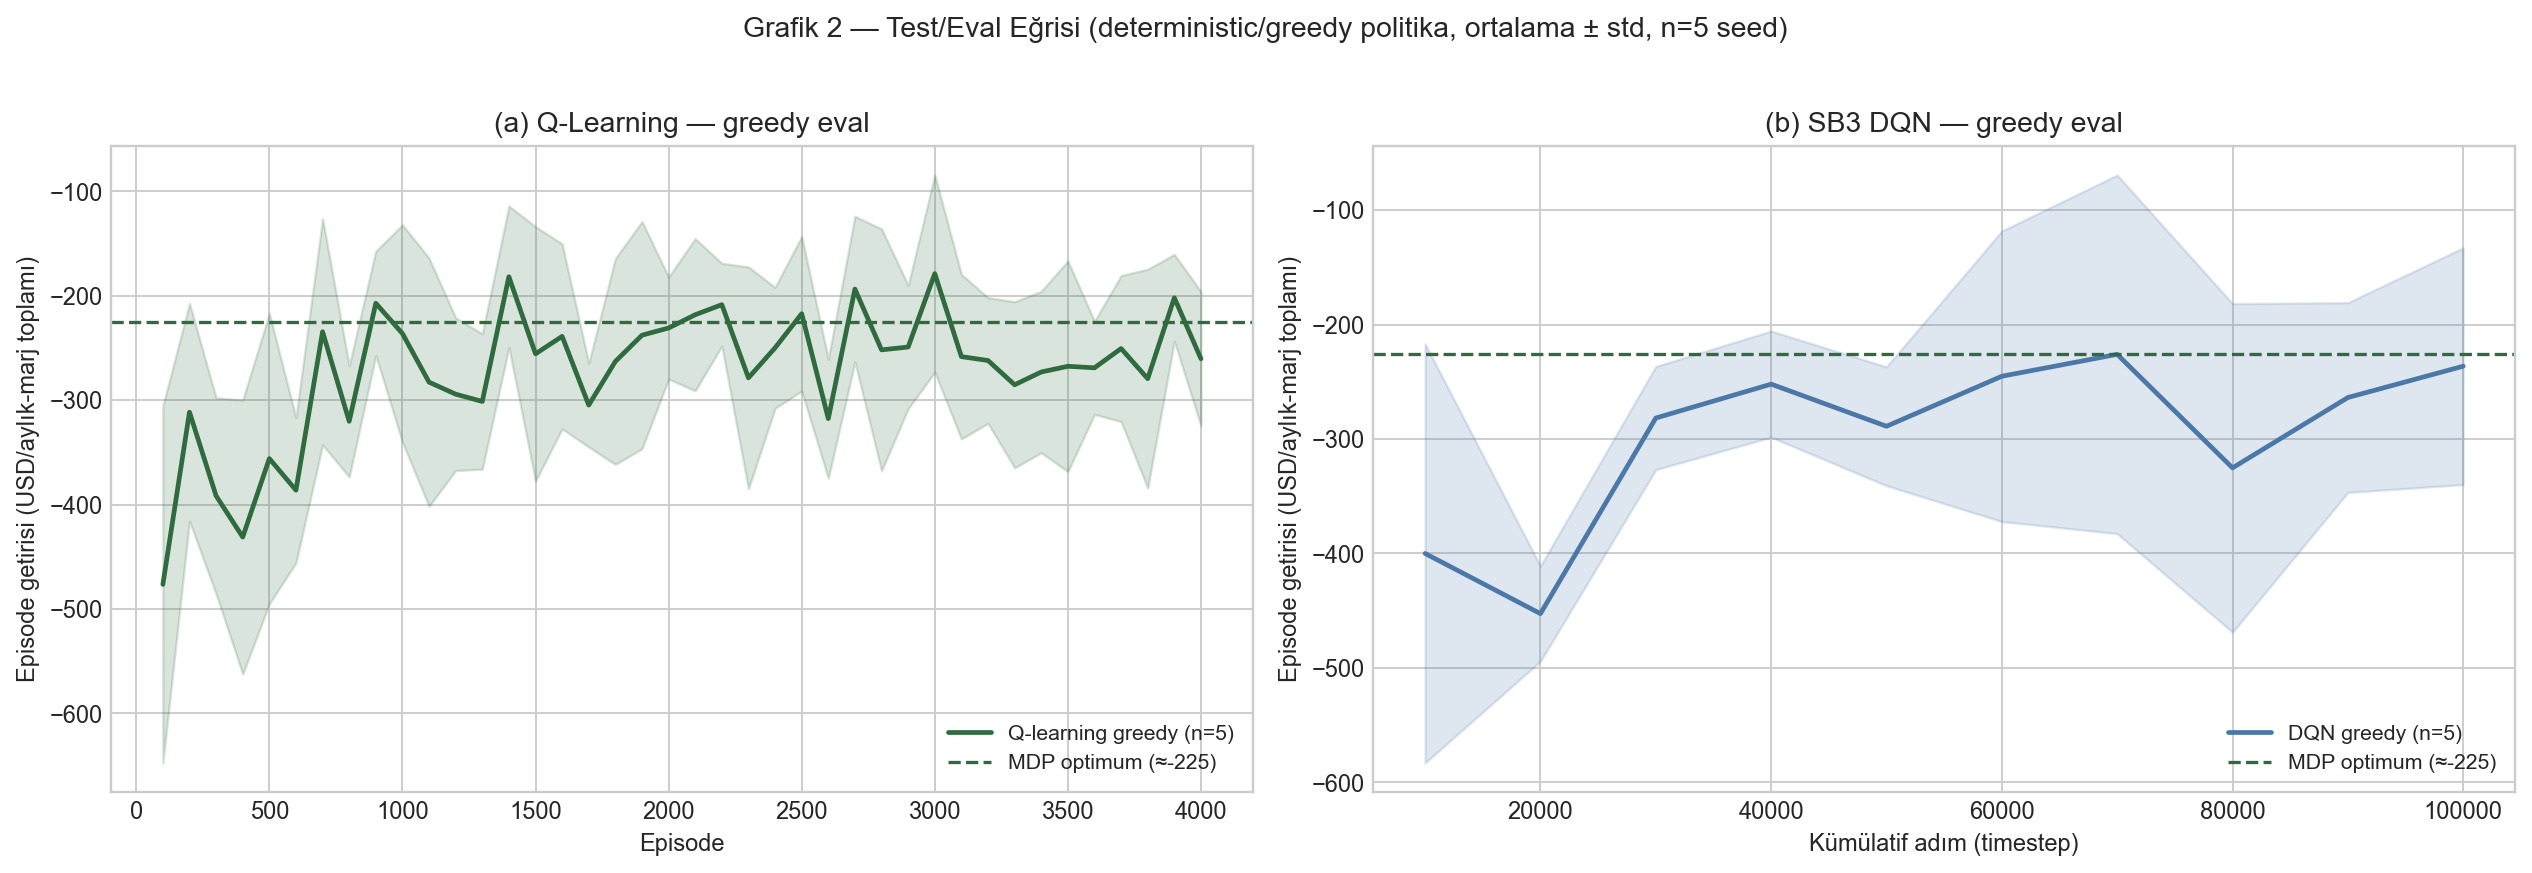
\includegraphics[width=0.92\textwidth]{02_eval_egrisi.png}
\caption{Değerlendirme eğrisi: deterministik/açgözlü politika; yeşil kesik çizgi VI
optimum referansı. $n\!=\!5$ tohum, ortalama$\pm$std.}
\label{fig:eval}
\end{figure*}

\subsection{Kayıp ve Politika Isı Haritası (Şekil \ref{fig:loss})}
Sol panelde DQN'in TD-kaybı, logaritmik eksende başlangıç değerinden hızla düşerek
yakınsar; bu, Q-hedefine doğru kararlı bir optimizasyonun göstergesidir. Tablo
yöntemlerinde kayıp bulunmadığından, sağ panelde Q-Learning'in öğrendiği politika bir ısı
haritasıyla verilir: risk bandı ve DIM'e göre ortalama cull oranı. Desen iktisadi olarak
beklendiği gibidir: yüksek riskli ve ileri laktasyondaki ineklerde cull eğilimi belirgin
biçimde artar. Hem optimizasyon dinamiği (kayıp) hem de karar yapısı (ısı haritası) bu
yüzden sağlıklı ve yorumlanabilirdir.

\begin{figure*}[t]
\centering
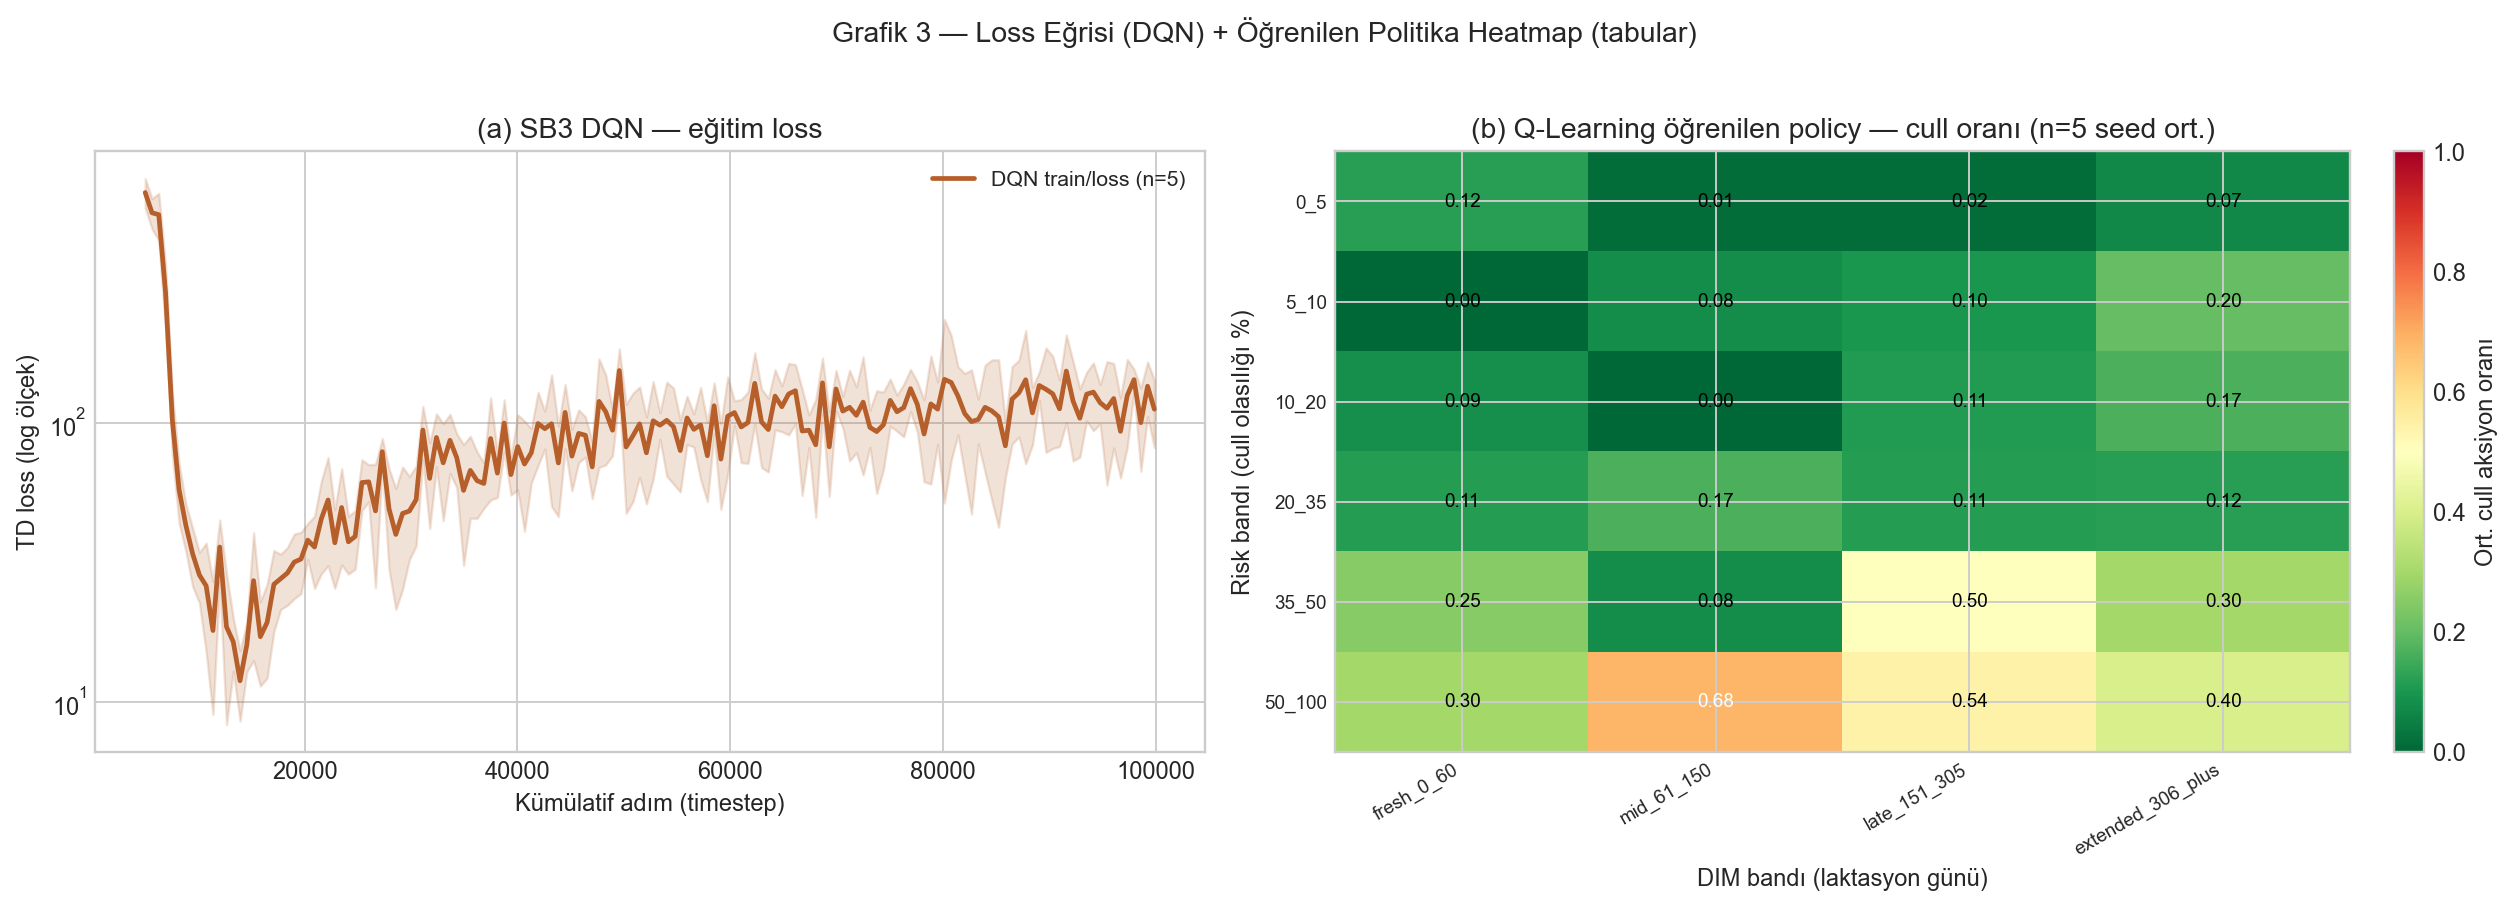
\includegraphics[width=0.92\textwidth]{03_loss_ve_policy_heatmap.png}
\caption{Sol: DQN eğitim kaybı (log eksen). Sağ: Q-Learning öğrenilen politikanın
risk$\times$DIM ısı haritası (ortalama cull oranı, $n\!=\!5$).}
\label{fig:loss}
\end{figure*}

\subsection{Hiperparametre Duyarlılığı (Şekil \ref{fig:hp})}
$\varepsilon_0\times\alpha$ ızgarası (3$\times$3, tohum başına tekrarlı) en yüksek getiriyi
orta düzey keşif ($\varepsilon_0\!=\!0.35$) ve orta düzey öğrenme oranında
($\alpha\!=\!0.18$) verir. Uç köşeler daha kötüdür: çok az keşif ajanı yeterince farklı
durumu görmeden erken sömürüye sıkıştırır, çok fazla keşif ise eğitim bütçesini rastgele
aksiyonlarda harcar; aşırı yüksek $\alpha$ ise güncellemeleri gürültüye aşırı duyarlı
kılarak yakınsamayı bozar. Bu klasik keşif--sömürü dengesidir. Seçilen varsayılanların
tam da bu en iyi hücreye denk gelmesi, konfigürasyonun keyfî değil veriyle gerekçeli
olduğunu gösterir.

\begin{figure*}[t]
\centering
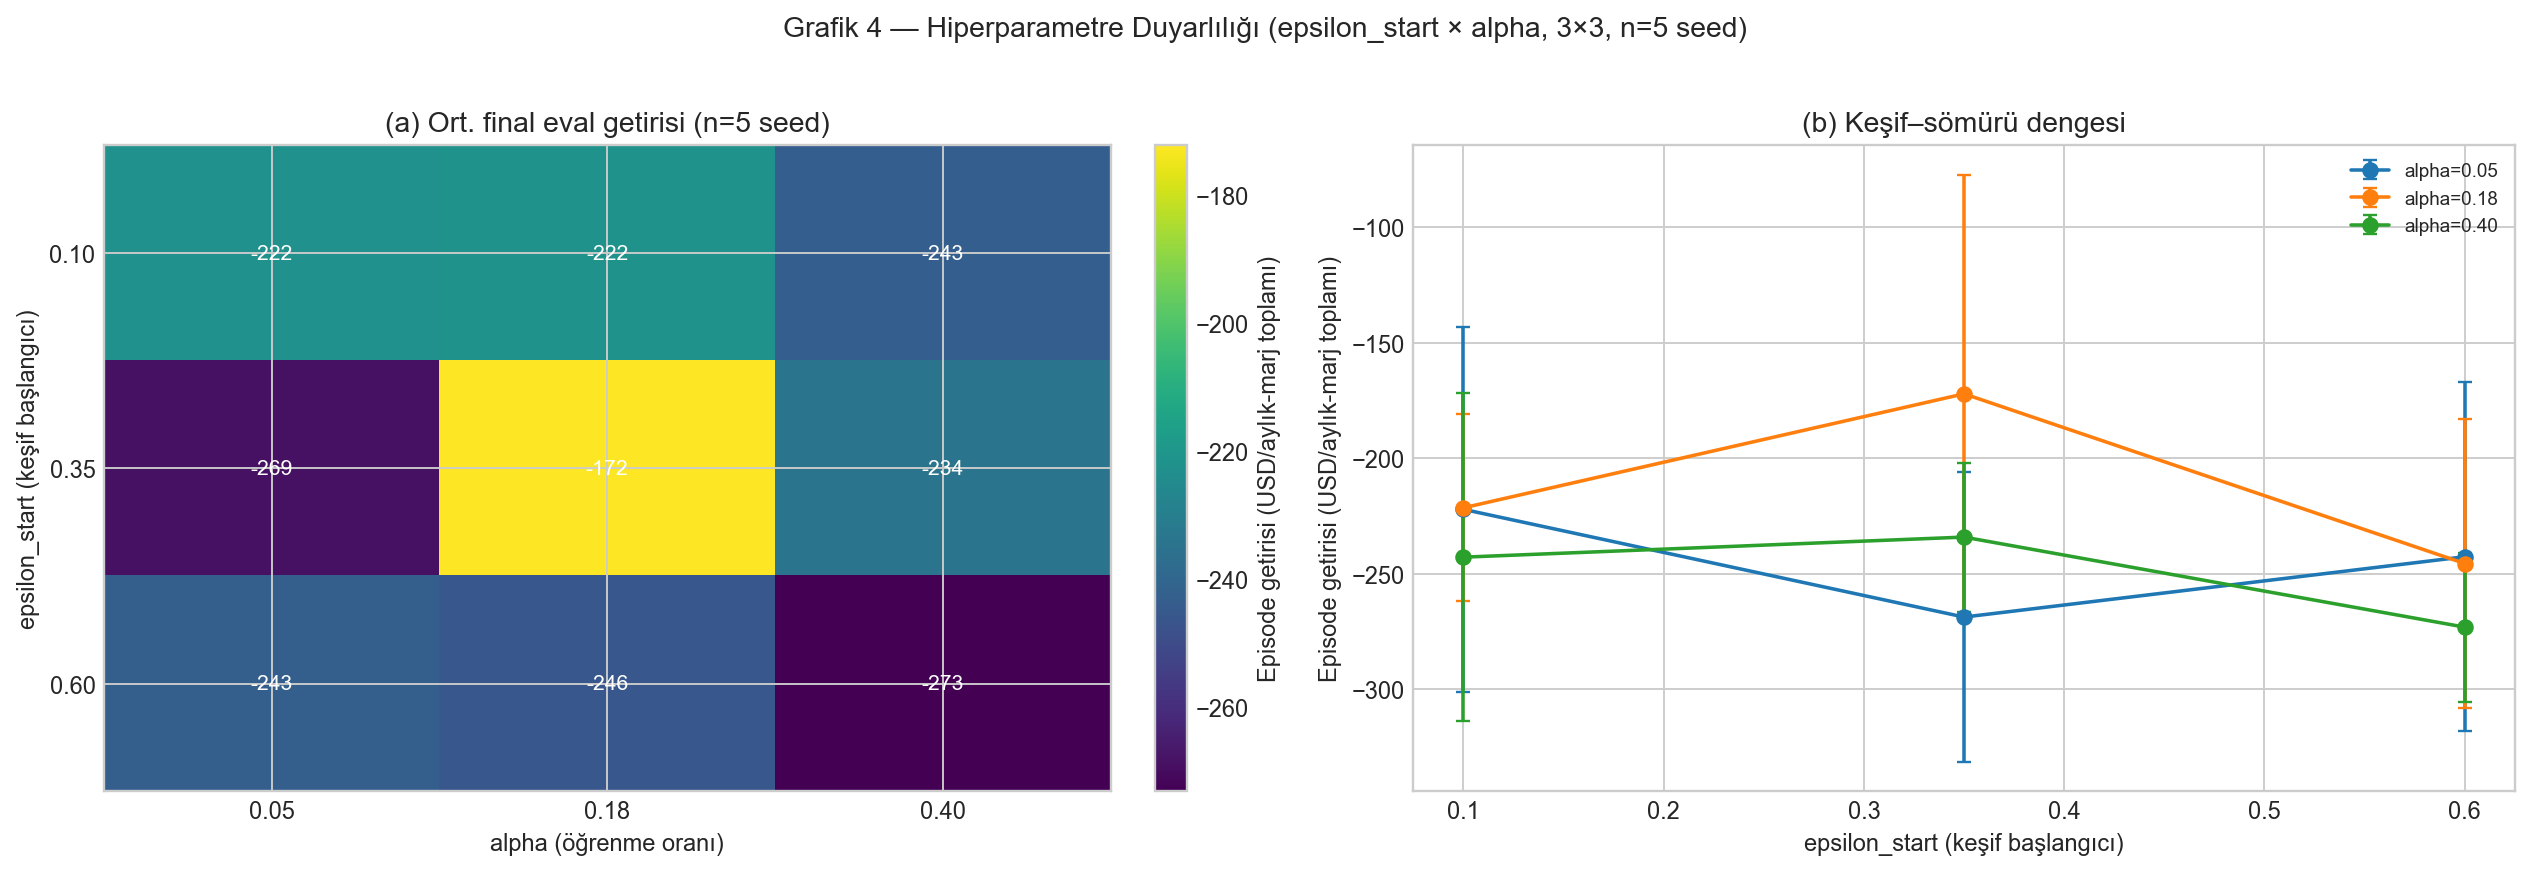
\includegraphics[width=0.92\textwidth]{04_hiperparametre_duyarlilik.png}
\caption{Hiperparametre duyarlılığı: $\varepsilon_0\times\alpha$ (3$\times$3), $n\!=\!5$
tohum. Sol: ortalama getiri ısı haritası. Sağ: keşif--sömürü eğrileri.}
\label{fig:hp}
\end{figure*}

\subsection{Baseline Karşılaştırması (Şekil \ref{fig:base})}
Final açgözlü değerlendirme getirisi, eğitilmiş ajanların (mavi) tüm naif ve heuristik
baseline'ları (turuncu) açık ara geçtiğini gösterir; VI optimum (yeşil) tavan referanstır.
Naif politikalar arasında \texttt{cull\_all} en kötüsüdür ($-1300$, her hayvanı hemen
çıkarmak değer yaratmaz), \texttt{random} ve \texttt{keep\_all} da düşüktür. Ajanların
gecikmeli ödülü ve stokastik geçişleri hesaba katması, miyop baseline'lara karşı ölçülebilir
bir iktisadi üstünlük sağlar. Hata çubukları ($\pm$std) bu üstünlüğün tohumlar arasında
tutarlı olduğunu doğrular ve böylece çevre seçimini gerekçelendirir.

\begin{figure}[t]
\centering
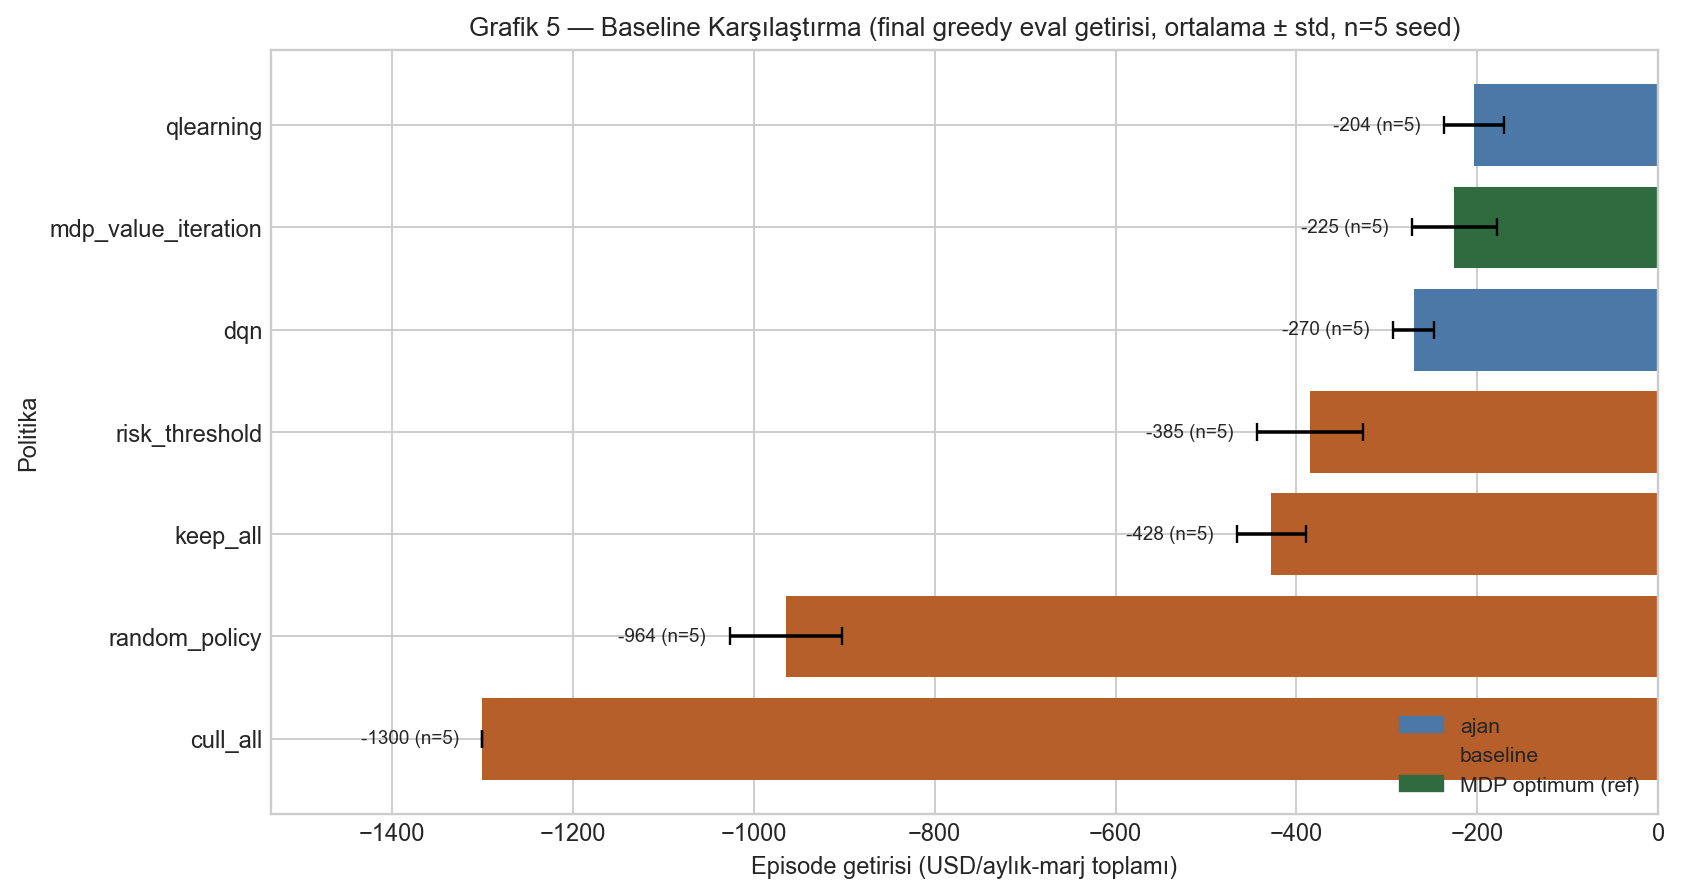
\includegraphics[width=\columnwidth]{05_baseline_karsilastirma.png}
\caption{Baseline karşılaştırması: final açgözlü değerlendirme getirisi
(ortalama$\pm$std, $n\!=\!5$). Mavi: ajan, turuncu: baseline, yeşil: VI optimum.}
\label{fig:base}
\end{figure}

\section{Kavramsal Analiz}
\textbf{Determinizm.} Ortam stokastiktir: \texttt{keep} için $p(s'\mid s,\text{keep})$
empirik bir dağılımdır (durumların $\%74$'ünde $>\!1$ olası $s'$;
\texttt{rl\_experiment\_utils.py:161}). Aynı tohumla aynı yörüngenin elde edilmesi yalnızca
tekrarlanabilirliği gösterir, dinamiğin deterministik olduğunu değil; başlangıç \emph{ve}
geçiş kuralı stokastiktir, \texttt{cull} ise deterministik terminaldir.

\textbf{On/Off-policy.} Q-Learning off-policy'dir: davranış $\varepsilon$-greedy
(\texttt{rl\_core.py:309}), hedef açgözlü $\max$ (\texttt{:321}). DQN de off-policy'dir ve
replay buffer kullanır (\texttt{:474}). Her ikisi de \emph{online} (simülatörle etkileşerek)
öğrenir; bu, on/off ayrımıyla karıştırılmamalıdır. Gerçek loglu davranış-politikası verisi
bulunmadığından CQL/IQL gibi gerçek offline yöntemler kapsam dışıdır.

\textbf{Markov.} Empirik geçiş modeli \texttt{state\_bucket}$\rightarrow$\texttt{next} olarak
Markov varsayımı altında kurulmuştur; süt trendi ve risk bandı geçmişi özetleyerek bu
varsayımı güçlendirir. Ancak ayrıklaştırma bilgi kaybı yarattığından özellik
\emph{yaklaşık} Markov'dur; tam gebelik günü veya hastalık şiddeti gibi ince bilgiler
durumda yer almaz.

\textbf{POMDP.} Gerçek durum (ineğin tam fizyolojisi) ile gözlem (aylık, ayrık, sensörle
sınırlı snapshot) ayrışır; \texttt{cull\_risk} gerçek bir etiket değil denetimli bir
\emph{tahmindir} \cite{kaelbling}. Trend ve risk özniteliklerinin eklenmesi (öznitelik
mühendisliği), gözlemi Markov'a yaklaştıran ve vanilla DQN'in kısmi gözlemlenebilirlik
sınırını hafifleten bir çözümdür; risk skoru bir tür sıkıştırılmış inanç (belief) gibi
davranır.

\section{Sınırlamalar}
\label{sec:limitations}
Süt fiyatı (0.4668) ve bakım maliyeti (8.5337) USDA~2025 kaynaklıdır; replacement, cull,
tedavi ve tohumlama maliyetleri prototip varsayımıdır
(\texttt{reward\_baseline\_us\_2025.csv}, \texttt{value\_source} sütunu). Politika bu
varsayımlara duyarlıdır; senaryo analizi bu duyarlılığı incelemek için mevcuttur.
Simülatör empirik bir MDP'dir, üretim politikası değildir. Gerçek loglu aksiyon
bulunmadığından offline RL ve sürekli-aksiyon yöntemleri bu fazda uygulanmamıştır.

\section{Sonuç}
Ardışık, gecikmeli-ödüllü ve stokastik bir keep/cull ortamı kurularak problemin RL
gerektirdiği gösterilmiş; model-free Q-Learning ve DQN ajanları $\geq5$ tohum üzerinde
tüm baseline'ları geçmiş ve model-tabanlı optimuma istatistiksel olarak eşitlenmiştir (fark anlamlı değildir). Ödül mekanizması
kaynak kodla birebir eşleşir, tüm sonuçlar ham loglardan doğrulanabilir ve tek komutla
yeniden üretilebilir. Gelecek çalışmada gerçek loglu aksiyonlarla offline RL ve daha zengin
durum gösterimleriyle POMDP yaklaşımları değerlendirilebilir.

\begin{thebibliography}{1}
\bibitem{sutton} R.~S.~Sutton ve A.~G.~Barto, \emph{Reinforcement Learning: An Introduction}, 2.~bs. MIT Press, 2018.
\bibitem{watkins} C.~J.~C.~H.~Watkins ve P.~Dayan, ``Q-learning,'' \emph{Machine Learning}, c.~8, ss.~279--292, 1992.
\bibitem{dqn} V.~Mnih \emph{ve di\u{g}.}, ``Human-level control through deep reinforcement learning,'' \emph{Nature}, c.~518, ss.~529--533, 2015.
\bibitem{gym} M.~Towers \emph{ve di\u{g}.}, ``Gymnasium,'' Zenodo, 2023.
\bibitem{sb3} A.~Raffin \emph{ve di\u{g}.}, ``Stable-Baselines3: Reliable reinforcement learning implementations,'' \emph{JMLR}, c.~22, 2021.
\bibitem{kristensen} A.~R.~Kristensen, ``Optimal replacement and ranking of dairy cows determined by a hierarchic Markov process,'' \emph{Livestock Production Science}, c.~16, ss.~131--144, 1987.
\bibitem{cabrera} V.~E.~Cabrera, ``A simple formulation and solution to the replacement problem: A practical tool to assess the economic cow value,'' \emph{J. Dairy Science}, c.~95, ss.~4683--4698, 2012.
\bibitem{kaelbling} L.~P.~Kaelbling, M.~L.~Littman ve A.~R.~Cassandra, ``Planning and acting in partially observable stochastic domains,'' \emph{Artificial Intelligence}, c.~101, ss.~99--134, 1998.
\end{thebibliography}

\end{document}
